% !TEX root = pfe-book1.tex
%!TEX TS-program = pdflatex
%!TEX encoding = UTF-8 Unicode


\cleardoublepage
\chapter{Gravitation}
\section{What Holds the Earth Up!}
In the distant past, people gave a simple answer to
this question: the three whales. True, it remained unclear
what was holding the whales up. However, this did not
disturb our na\"ive forefathers.

Correct ideas about the nature of the Earth's motion,
the Earth's form and many regularities in the motion of
the planets around the Sun had arisen long before an
answer was given to the question of the causes for the
motion of the planets.

And really, what ``holds up'' the Earth and the planets? Why do they move around the Sun along definite
paths instead of flying away from it?

There was no answer to these questions for a long time,
and the Church, struggling against the Copernican system of the Universe, used this to negate the fact of the
Earth's motion.

We are obliged to the great English scientist Isaac Newton for his discovery of the true answers.

A well-known historical anecdote asserts that while
sitting in an orchard under an apple-tree, thoughtfully
observing how one apple after another fell to the ground
because of gusts of wind, Newton arrived at the idea of
the existence of gravitational forces between all bodies
in the Universe.

As a result of Newton's discovery, it became clear that
many apparently miscellaneous phenomena -- the free
fall of bodies to the Earth, the apparent motions of the Moon and the Sun, the ocean tides, etc. -- are manifestations of one and the same law of nature -- the law of universal gravitation.

Between all bodies in the Universe, asserts this law,
be they grains of sand, peas, stones or planets, forces of
mutual attraction are exerted.

At first sight, this law seems false: we somehow haven't
noticed that the objects surrounding us were attracted to each other. The Earth attracts all bodies to itself;
no one will have any doubt about this. But perhaps this
is a special property of the Earth? No, that isn't so. The
attraction of two arbitrary objects is slight, and this is
the only reason why it doesn't arrest our attention. Nevertheless, it can be detected by means of special experiments. But more about that later.

The presence of universal gravitation, and nothing else,
explains the stability of the solar system and the motion
of the planets and other celestial bodies.

The Moon is kept in orbit by terrestrial gravitational
forces, and the Earth on its trajectory by solar gravitational forces.

The circular motion of celestial bodies occurs in the
same way as the circular motion of a stone twirled on
a string. The forces of universal gravitation are invisible
``ropes'' compelling celestial bodies to move along definite
paths.

The assertion of the existence of universal gravitational
forces didn't really mean much. Newton discovered the
law of gravitation and showed what these forces depend
on.

\section{Law of Universal Gravitation}
The first question which Newton asked himself was the
following: How does the Moon's acceleration differ from
that of an apple? To put it otherwise, what is the difference between the acceleration $g$ which the Earth creates
on its surface, i.e. at the distance $r$ from its centre, and
the acceleration created by the Earth at the distance $R$
at which the Moon is located from the Earth?

In order to calculate this acceleration, $v^{2}/R$, it is necessary to know the speed of the Moon's motion and its
distance from the Earth. Both these figures were known
by Newton. The Moon's acceleration turned out to be
approximately equal to \SI{0.27}{\centi\meter\per\second\squared}. This is about 3600
times less than the value of $g$,  \SI{980}{\centi\meter\per\second\squared}.

Hence, the acceleration created by the Earth decreases
as one recedes from the centre of the Earth. But how rapidly? The distance from the Earth to the Moon equals
sixty terrestrial radii. But 3600 is the square of 60. Increasing the distance by a factor of 60, we decrease the
acceleration by a factor of $60^{2}$.

Newton concluded that the acceleration, and therefore
also the gravitational force, is inversely proportional to
the square of the distance. Further, we already know that
the force exerted on a body in a gravitational field is proportional to its mass. Therefore, the first body attracts
the second with the force proportional to the mass of the
second body; the second body attracts the first with the
force proportional to the mass of the first body.

We are dealing with identically equal forces -- forces of
action and reaction. Consequently, the mutual gravitational force must be proportional to the mass of the first
body as well as to that of the second or, to put it otherwise, to the product of the masses.

Thus,
 \begin{equation*}%
F =  G  \, \dfrac{Mm}{r^{2}}
 \end{equation*}
 This is precisely the \emph{law of universal gravitation}. Newton
assumed that this law will be valid for any pair of bodies.

This bold hypothesis is now completely proved. Therefore, the force of attraction between two bodies is directly proportional to the product of their masses and inversely proportional to the square of the distance between them.

But what is this $G$ that entered the formula? This is the coefficient of proportionality. May we assume it to be equal to unity, as we have already repeatedly done? No, we may not: we have agreed to measure mass in grams, distance in centimetres, and force in dynes. The value of $G$ is equal to the force of attraction between two masses of \SI{1}{\gram} located at a distance of \SI{1}{\centi\meter} from each other. We cannot assume that the force is equal to anything (in particular, to one dyne). The coefficient $G$ must be measured.

In order to find $G$, we don't, of course, have to measure the forces of attraction between gram weights. We are interested in carrying out measurements on massive bodies -- the force will be greater then.

If we determine the mass of two bodies, know the distance between them and measure the force of attraction,
then $G$ will be found by a simple calculation.

Such experiments were performed many times. They showed that the value of $G$ is always one and the same, independent of the material of the attracting bodies and also of the properties of the medium in which they are situated. The quantity G is called the \emph{gravitational constant}. It is equal to \SI{6.67e-8}{\centi\meter\cubed\per\gram\per\second\squared}.

 \begin{figure}[!ht]
 \centering
 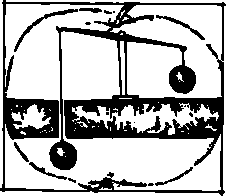
\includegraphics[width=0.6\textwidth]{figures/fig-6-1.pdf}
 \caption{An experiment to determine universal constant of gravitation.}
 \label{fig-6-1}
 \end{figure}
The diagram of one of the experiments on measuring
$G$ is shown in the diagram above \figr{fig-6-1}. Two balls of identical mass are
suspended from the ends of a beam of scales. One of them
is situated above a lead plate, the other beneath it. By
means of its attraction, the lead (100 tons of it are taken
for the experiment) increases the weight of the ball on the
right and decreases that of the ball on the left. The former outweighs the latter. The value of $G$ is computed on the
basis of the magnitude of the deflection of the beam.

The difficulty in detecting gravitational forces between two objects is explained by the negligible value of $G$.
Two heavy \SI{1000}{\kilo\gram} loads pull each other with a negligible force equal in all to only \SI{6.7}{\dyne}, i.e. 0.007~gf, if these
objects are situated, say, at a distance of \SI{1}{\meter} from each other.

But how great are the forces of attraction between celestial bodies? Between the Moon and the Earth
 \begin{align*}%
F & =  \num{6.7e-8} \times \dfrac{\num{6e27} \times 0.74 \times \num{d26}}{(\num{38e9})^{2}}  = \SI{2e25}{\dyne} \approx \SI{2e19}{\kgf}\\
& \text{and between the Earth and the Sun}\\
F & =  \num{6.7e-8} \times \dfrac{\num{2e33} \times 6 \times \num{d27}}{(\num{15e12})^{2}}  = \SI{3.6e27}{\dyne} \approx \SI{3.6e21}{\kgf}
 \end{align*}

\section{Weighing the Earth}

Before beginning to make use of the law of universal
gravitation, we must turn our attention to an important
detail.

We have just calculated the force of attraction between
two loads located at a distance of \SI{1}{\meter} from each other.
But if this distance were \SI{1}{\centi\meter}? What would we then substitute in the formula -- the distance between the surfaces
of bodies or the distance between their centres of gravity
or some other value?

The law of universal gravitation, $F = G \, m_{1}m_{2}/r^{2}$, can
be applied with complete rigour when such doubts do not
arise. The distance between the bodies should be much
greater than their dimensions; we should have the right
to regard the bodies as points. But how should we apply
the law to two nearby bodies? This is simple in principle:
we must conceptually break up the bodies into small
pieces, calculate the force $F$ for each pair and then add
(vectorially) all the forces.

In principle this is simple, but it is rather complicated
in practice.

However, nature has helped us. Computations show that
if the particles of a body interact with a force proportional to $1/r^{2}$, spherical bodies possess the property of attracting like points located at the centres of the spheres. For two nearby spheres, the formula $F = G \,m_{1}m_{2}/r^{2}$ is exactly
valid, just as for distant spheres, if $r$ is the distance between their centres. We have already used this rule above
in computing the acceleration on the Earth's surface.

We now have the right to apply the gravitational formula for computing the forces with which the Earth
attracts bodies. We should take the distance from the
centre of the Earth to the body as $r$. Let $M$ be the mass, and $R$ the radius of the Earth. Then the force of attraction acting on a body of mass $m$ at the Earth's surface
 \begin{equation*}%
F = G \, \dfrac{m_{1}m_{2}}{r^{2}}
 \end{equation*}
But this is in fact the body's weight, which we always
express as $mg$. Hence, the acceleration of free fall
 \begin{equation*}%
g = G \, \dfrac{M}{R^{2}}
 \end{equation*}
 Now at last we can say how the Earth was weighed.
The quantities $g$, $G$ and $R$ are known, so the Earth's
mass can be computed from this formula. The Sun can
also be weighed in the same manner.

But can we really call such a procedure weighing?
Of course we can; indirect measurements play at least
as great a role in physics as direct measurements.

Let us now solve a curious problem.

An essential role in the plans for creating world-wide
television is played by the creation of a ``24-hour satellite'', i.e. one which will always be situated over one
point on the Earth's surface. Will such a satellite experience a significant frictional force? This depends on
how far from the Earth it will have to perform its rotation.

A 24-hour satellite should revolve with a period $T$
equal to 24 hours. If $r$ is the distance from the satellite
to the centre of the Earth, then its speed $v = 2 \pi r/T$
and its acceleration 
 \begin{equation*}%
\dfrac{v^{2}}{r} =  \dfrac{4 \pi^{2} \, r}{T}
 \end{equation*}
On the other hand, this acceleration whose source is the Earth's attraction
is equal to 
 \begin{equation*}%
\dfrac{GM}{r^{2}}= \dfrac{gR^{2}}{r^{2}}
 \end{equation*}
Equating our two expressions for the acceleration, we obtain:
 \begin{equation*}%
g \, \dfrac{R^{2}}{r^{2}}=  \dfrac{4 \pi^{2} \, r}{T^{2}} \quad \textrm{i.e.} \quad r^{3} =   \dfrac{g R^{2} T^{2}}{4 \pi^{2}} 
 \end{equation*}
Substituting the founded-off values of $g = \SI{10}{\meter\per\second\squared}$,
$R = \SI{6e6}{\meter}$ and $T = \SI{9e4}{\second}$, we obtain: 
 \begin{equation*}%
r^{3} = \SI{7e22}{\meter\cubed}, \,\, \textrm{i.e.} \,\, r \approx \SI{4e7}{m} =  \SI{40000}{\kilo\meter} 
\end{equation*}
 There is no air friction at such a height, and a 24-hour satellite will not slow down its ``motionless orbiting''.
	
\section{Measuring \emph{g} in the Service of Prospecting}

The topic is geological prospecting whose aim is to find deposits of useful minerals under the Earth without
digging a pit or sinking a shaft.

 \begin{figure}[!ht]
 \centering
 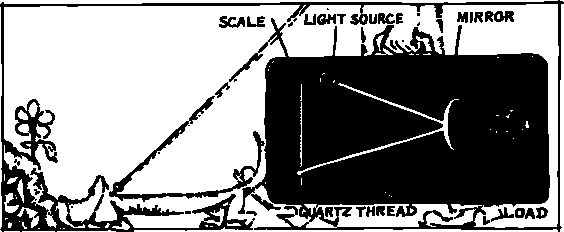
\includegraphics[width=\textwidth]{figures/fig-6-2.pdf}
 \caption{An extremely sensitive geological balance with a quartz thread.}
 \label{fig-6-2}
 \end{figure}

There exist several methods of determining the acceleration of free fall very accurately. It is possible to
find $g$ by simply weighing a standard weight on a spring balance. Geological balances should be extremely sensitive their spring -- changes its tension when a load of less than a millionth of a gram is added. Quartz torsion
balances yield excellent results. Their construction isn't
complicated in principle. To a horizontally stretched
quartz thread a lever is welded whose weight slightly
twists the thread \figr{fig-6-2}.

A pendulum is used for the same purposes. Not very
long ago pendulum methods of measuring $g$ were the
only ones, and only in the last 10-20 years have the more
convenient and precise balance methods begun to supplant
them. In any case, measuring the period of oscillation
of a pendulum one can find the value of $g$ accurately enough from the formula $T = 2 \pi \sqrt{l/g}$.

Measuring values of $g$ at different places with the same
apparatus, we can detect relative changes in the free
fall up to one-millionth.

Measuring the value of $g$ at some place on the Earth's
surface, the experimenter ascertains: here the value is
anomalous, it is so much less than the norm or such an
amount greater than the norm.

But what is the norm for the value of $g$?

There are two natural changes which have long been
observed and are well known to researchers in the value
of the acceleration of free fallon the Earth's surface.

First of all, $g$ decreases from a pole to the equator.
This has been spoken of above. Let us only recall that
such a change occurs as a result of two causes: firstly,
the Earth isn't a sphere, and a body at a pole will be
nearer to the centre of the Earth; secondly, the more a body
advances towards the equator, the more will the force
of gravity be weakened by the centrifugal force.

The second change in $g$ is the decrease due to elevation.
The greater the distance from the Earth's centre, the
smaller will be the value of $g$ in accordance with the
formula $g = GM/(R + h)^{2}$, where $R$ is the radius of the
Earth, and $h$ is the height above sea level.

Therefore, at one and the same latitude and at one and
the same height above sea level, the acceleration of free
fall should be identical.

Accurate measurements show that deviations from
this norm -- gravitational anomalies -- are found quite often. The cause of an anomaly consists in the heterogeneity of the mass distribution near the place of measurement.

As we explained, the gravitational force due to a large
body can be conceptually represented as the sum of forces
emanating from the individual particles of the large body.
The attraction of a pendulum to the Earth is the result
of the action of all the particles of the Earth on it. But
it is clear that the nearby particles make the greatest
contribution to the resultant force, for the attraction
is inversely proportional to the square of the distance.

If heavy masses are concentrated near the place of
measurement, $g$ will be greater than the norm; in the
opposite case, $g$ will be smaller than the norm.

If, for example, we measure $g$ on a mountain and in an
airplane flying over a sea at an altitude equal to the
mountain's height, a greater value will be obtained in
the former case. For example, the value of $g$ is \SI{0.292}{\centi\meter\per\second\squared}
greater than the norm on Mount Etna in Italy. The value
of $g$ is also higher than the norm on isolated ocean islands.
It is clear that in both cases the growth of $g$ is explained
by the concentration of additional masses at the place
of measurement.

Not only the value of $g$ but also the direction of the
force of gravity can deviate from the norm. If a load
is suspended on a thread, the stretched thread will indicate the vertical for the given place. This vertical may
deviate from the norm. A normal vertical can be determined by the stars, since it has been calculated for any
geographical point at what place in the sky the vertical
to the ``ideal'' form of the Earth is ``set'' at a given instant
of a day and year.

Imagine that you are performing experiments with
a plumb-line at the foot of a large mountain. The load of
the plumb-line is attracted by the Earth towards its
centre, and by the mountain to one side. Under such
conditions, the plumb-line must be deflected from the
direction of a normal vertical (\figr{fig-6-3}). Since the
Earth's mass is much greater than that of the mountain,
such a deflection will not exceed several seconds of arc.
Plumb-line deflections sometimes yield strange results.
For example, in Florence the influence of the Appenines
leads not to an attraction, but to a repulsion of a plumb-line. The explanation can only be as follows: there are
enormous empty spaces in mountains.
 \begin{figure}[!ht]
 \centering
 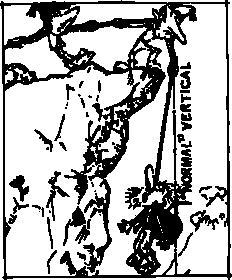
\includegraphics[width=0.45\textwidth]{figures/fig-6-3.pdf}
 \caption{Plumb line deflections from the normal vertical.}
 \label{fig-6-3}
 \end{figure}
Measurements of the acceleration of free fall to the
scale of continents and oceans yield remarkable results.
Continents are considerably heavier than oceans; therefore,
it would seem that the values of $g$ over continents should:
be greater than those over oceans. But in reality, the
values of $g$ measured along a single latitude over oceans
and continents are identical, on the average. Again there
is only one explanation: continents lie on lighter bedrocks, and oceans on heavier ones. And as a matter of
fact, where direct prospecting is possible, geologists
ascertain that oceans lie on heavy basaltic bed-rocks,
and continents on light granite ones.

But the following question immediately arises: Why do
heavy and light bedrocks compensate so exactly for the
difference in weight between continents and oceans? Such
a compensation cannot be a matter of chance; its cause
must be rooted in the construction of the Earth's shell.

Geologists assume that it is as though the upper layers
of the Earth's shell were floating on an underlying plastic
(i.e. easily deformed like wet clay) mass. The pressure
at depths of about \SI{100}{\kilo\meter} should be identical everywhere,
just as the pressure at the bottom of a vessel filled with
water in which pieces of wood of various weights are
floating is identical everywhere. Consequently, a column
of matter with an area of \SI{1}{\meter\squared} from the surface to a depth
of \SI{100}{\kilo\meter} should have the same weight under an ocean
and under a continent.

This levelling of pressures (it is called isostasy) is just
what leads to the situation where along a single latitude
over oceans and continents the values of the acceleration
of free fall $g$ do not differ significantly.

Local gravitational anomalies serve us just as the
magic wand, which banged on the ground where there
was gold or silver, served little Mook in Hauf's fairy-tale.

One must look for heavy ore in those places where $g$ is
maximum. On the contrary, light salt deposits are discovered by finding localities with lowered values of $g$.
It is possible to measure $g$ with an accuracy up to a hundred-thousandth of \SI{1}{\centi\meter\per\second\squared}.

Prospecting with the aid of pendulums and super-exact
scales is called gravitational. It is of great practical
value, in particular when looking for oil. The fact is
that with gravitational prospecting, it is easy to discover
underground salt domes. It so happens that often oil is
found at those places too. Moreover, the oil lies at some
depth, while the salt is nearer to the Earth's surface.
Oil was discovered in Kazakhstan and in other places
by gravitational prospecting.

\section{Weight Underground}

It remains for us to throw light on another interesting
question. How will the force of gravity change if we go
deep underground?

The weight of an object is the result of the tension in,
so to say, invisible ``threads'' reaching out to this object
from every piece of matter in the Earth. Weight is the
resultant force, the result of the addition of the elementary forces exerted on the object by the Earth's particles.
All these forces, even though directed at different angles,
pull a body ``down'' -- towards the centre of the Earth.
 \begin{figure}[!ht]
 \centering
 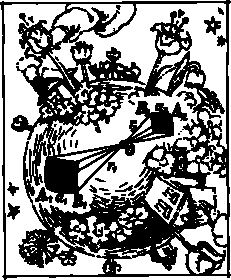
\includegraphics[width=0.45\textwidth]{figures/fig-6-4.pdf}
 \caption{Analysing gravitational forces on a point inside the surface of the Earth.}
 \label{fig-6-4}
 \end{figure}
But what will be the weight of an object in an underground laboratory? Forces of attraction will be exerted
on it both by the internal and external layers of the
Earth.

Consider the gravitational forces exerted at a point
lying inside the Earth by an external layer. If we break
up this layer into thin shells, cut out in one of them a
small square with side $a_{1}$ and draw lines from the vertices
of the square through the point $O$ (we are interested in
the weight at those points), then on the opposite side
of the shell we obtain a small square of a different size
with side $a_{2}$ (\figr{fig-6-4}). The forces of attraction exerted
at the point $O$ by the two small squares are oppositely
directed and proportional according to the law of gravitation to $m_{1}/r_{1}^{2}$ and $m_{2}/r_{2}^{2}$. But the masses of the squares,
$m_{1}$ and $m_{2}$ , are proportional to their areas. Therefore the gravitational forces are proportional to the expressions $a_{1}^{2}/r_{1}^{2}$ and $a_{2}^{2}/r_{2}^{2}$.

I suggest that the reader prove that these ratios are the
same, that is, that the forces of attraction at point $O$
acting from the two small squares balance.

Having broken up a thin shell into pairs of ``opposite''
similar squares, we established a remarkable fact: a thin
homogeneous spherical shell does not act on a point
within it. But this is true for all the thin shells into which
we broke up the spherical layer lying above the underground point we are interested in.

Hence, the layer of the Earth lying above the body
might just as well be absent. The action of its individual
parts on the body is neutralized, and the resultant force
of attraction exerted by the external layer is equal
to zero.

Of course, throughout this reasoning we have assumed
the Earth's density to be constant within each shell.

The result of our reasoning permits us to easily obtain
a formula for the gravitational force exerted at any
depth $H$ under the Earth. A point situated at depth $H$
only experiences the attraction exerted by the internal
layers of the Earth. The formula for the acceleration due
to gravity, $g = GM/R^{2}$ , also applies to this case, where $M$
and $R$ are the mass and radius not of the entire Earth
but of its ``internal'' part with respect to this point.
If the Earth had the same density in all its layers, the
formula for $g$ would assume the following form:
 \begin{equation*}%
g = G \, \dfrac{\dfrac{4}{3} \pi \rho \, (R - H)^{3}}{(R - H)^{2}} = \dfrac{4}{3} \, \pi \, G \rho \, (R - H)
 \end{equation*}
where $\rho$ is the density, and $R$ is the Earth's radius.

This implies that $g$ would be directly proportional to
$(R - H)$: the greater the depth $H$, the smaller would be $g$.

But as a matter of fact, the behaviour of $g$ near the
Earth's surface -- we are able to observe it up to a depth
of \SI{5}{\kilo\meter} (below sea level) -- does not obey this law at all. Experiments show that $g$, on the contrary, increases with
depth within these layers. The lack of agreement between
the experiments and our formula is explained by the fact
that the difference in density at various depths was not
taken into account.

The average density of the Earth is easily found by
dividing its mass by its volume. This yields a value of
5.52. At the same time, the density of the surface bedrocks is much smaller -- it is equal to 2.75. The density
of the Earth's layers increases with depth. Within the
surface layers of the Earth, this effect dominates the
ideal decrease which follows from the formula just derived, and so the value of $g$ increases.

\section{Gravitational Energy}

We have already become acquainted with gravitational
energy through a simple example. A body raised to
height $h$ above the Earth possesses potential energy $mgh$.

However, this formula may be used only when height
$h$ is much smaller than the Earth's radius.

Gravitational energy is an important quantity, and
it would be interesting to obtain a formula for it which
would apply to a body raised to an arbitrary height above
the Earth and also, more generally, for two masses
attracting each other in accordance with the universal
law:
 \begin{equation*}%
F  = G\, \dfrac{m_{1}m_{2}}{r^{2}} 
 \end{equation*}
Let us assume that the bodies approached each other
somewhat under the action of their mutual attraction.
The distance between them was $r_{1}$, but it became $r_{2}$.
Moreover, the work $ A = F (r_{1} - r_{2} )$ is performed. The
value of the force must be taken at some intermediate
point. Thus,
 \begin{equation*}%
A =  G \,  \dfrac{m_{1}m_{2}}{r_{\textrm{int}}^{2}} \, (r_{1} - r_{2} )
 \end{equation*}
 If $r_{1}$ and $r_{2}$ do not differ much, we may replace $r_{\textrm{int}}$ by the
product $r_{1}r_{2}$. We obtain:
 \begin{equation*}%
A =  G \, \dfrac{m_{1}m_{2}}{r_{2}} -  G  \, \dfrac{m_{1}m_{2}}{r_{1}}
 \end{equation*}
This work is performed at the expense of the gravitational
energy:
 \begin{equation*}%
A =  U_{1} - U_{2}
 \end{equation*}
where $U_{1}$ is the initial and $U_{2}$ the final value of the
gravitational potential energy.

Comparing these two formulas, we find the following
expression for the potential energy:
 \begin{equation*}%
U = - \, G \,  \dfrac{m_{1}m_{2}}{r}
 \end{equation*}
It resembles the formula for the gravitational force,
but $r$ is raised to the first power in the denominator.

According to this formula, the potential energy $U = 0$
for very large $r$'s. This is reasonable, since the attraction
will no longer be felt at such distances. But when the
bodies approach each other, the potential energy should
decrease. After all, the work takes place at its expense.
But in what direction can it decrease from zero? In the
negative direction. Hence there is a minus sign in the
formula. After all, -5 is less than zero, and -10 is less
than -5.

If we are dealing with motion near the Earth's surface,
we may replace the general expression for the gravitational force by $mg$. Then with greater accuracy we have
 \begin{equation*}%
U_{1} = U_{2} =mgh
 \end{equation*}
But on the Earth's surface, a body has potential energy
$- \, GMm/R$, where $R$ is the Earths radius. 'Therefore,
at height $h$ above the Earth's surface,
 \begin{equation*}%
U = - \, G \, \dfrac{Mm}{R} +  mgh
 \end{equation*}
 
 When we first introduced the formula for potential
energy, $U = mgh$, we agreed to measure height and
energy from the Earth's surface. Using the formula
$U = mgh$, we discard the constant term $- \, GMm/R$,
regarding it as conditionally equal to zero. Since we are
interested only in energy differences, for it is work which
is an energy difference that is ordinarily measured, the
presence of the constant term $- \, GMm/R$ in the potential
energy formula does not play any role.

Gravitational energy determines the strength of the
``chains'' binding a body to the Earth. How can we break
these ``chains''? How can we ensure that a body thrown
from the Earth will not return to the Earth? It is clear
that to do this we must impart a large initial velocity
to the body. But what is the minimum velocity that is
required.

As a body (missile, rocket) thrown from the Earth
increases its distance from the Earth, its potential energy
will rise (the absolute value of $U$ will fall); its kinetic
energy will fall. If its kinetic energy becomes equal to
zero prematurely, before we break the Earth's gravitational ``chain'', the missile that was thrown will fall
back to the Earth.

It is necessary for the body to conserve its kinetic
energy until its potential energy practically vanishes.
Before its departure, a missile had potential energy
$- \,GMm/R$ ($M$ and $R$ are the mass and radius of the
Earth). Therefore, the missile must be given the velocity
which would make its total energy positive. A body with
a negative total energy (the magnitude of its potential
energy is greater than that of its kinetic energy) will
not get beyond the bounds of gravity.

Hence, we arrive at the simple condition. In order for
a body of mass $m$ to break away from the Earth, it must,
as has been already said, overcome the gravitational
potential energy
 \begin{equation*}%
G \, \dfrac{Mm}{R}
 \end{equation*}
For this, the speed of the missile should be increased
to the value of the escape velocity from the Earth, $v_{2}$ ,
which is easily computed .By equating its kinetic and
potential energies:
 \begin{equation*}%
\dfrac{mv_{2}^{2}}{2}  = G \, \dfrac{Mm}{R}, \quad \textrm{i.e.} \quad v_{2}^{2} = 2G \, \dfrac{M}{R}
 \end{equation*}
or, since $g = GM/R^{2}$,
 \begin{equation*}%
v_{2}^{2} = 2 gR 
 \end{equation*}

The value of $v_{2}$ computed by means of this formula is
\SI{11}{\kilo\meter\per\second}, of course, without taking air resistance into
account. This speed is $\sqrt{2} = 1.41$ times as great as the orbital velocity $v_{1} \, \sqrt{gR}$ of an artificial satellite whose orbit is near the Earth's surface, i.e. $v_{2} = \sqrt{2v_{1}}$.

The mass of the Moon is 81 times as small as that of
the Earth; the radius of the Moon is four times as small
as that of the Earth. Consequently, the gravitational
energy on the Moon is twenty times less than that on the
Earth, and a speed of \SI{2.5}{\kilo\meter\per\second} is sufficient to break away
from the Moon.

Kinetic energy $mv^{2}_{2}/2$ is spent in order to break the
gravitational ``chains'' to the planet -- the take-off station.
If we want the rocket which has overcome gravity to
move with speed $v$, then additional energy $mv^{2}/2$ is needed
for this. In such a case, when launching the rocket, it is
necessary to impart it energy 
 \begin{equation*}%
\dfrac{mv^{2}_{0}}{2} = \dfrac{mv^{2}_{2}}{2} + \dfrac{mv^{2}}{2}    
 \end{equation*}
Therefore, the three speeds in question are connected by
the simple relation:
 \begin{equation*}%
v_{0}^{2} = v_{2}^{2} + v^{2}
 \end{equation*}
What should be the speed $v_{3}$ necessary for overcoming
the gravitation of the Earth and the Sun -- the minimum
speed of a missile sent to distant stars? We denoted this
speed by $v_{3}$ because it is called the escape velocity from
the solar system.

First of all, let us determine the speed necessary for
overcoming only the single attraction of the Sun.

As we have just shown, the speed needed to escape
from the Earth's attraction by a missile sent on a flight
is $\sqrt{2}$ times as great as the speed with which an Earth
satellite is sent into orbit. Our reasoning is equally valid
or the Sun, i.e. the speed needed to escape from the Sun
is $\sqrt{2}$ times as great as the speed of a satellite of the Sun
(i.e. the Earth). Since the speed of the Earth's motion
around the Sun is about \SI{30}{\kilo\meter\per\second}, the speed needed to
escape from the sphere of the Sun's attraction is \SI{42}{\kilo\meter\per\second}.
This is a very great speed, but for sending a missile to
distant stars, we must, of course, use the Earth's motion
and launch the body in the direction in which the Earth
is moving. We then need to add only $42 - 30 = \SI{12}{\kilo\meter\per\second}$.

Now we can finally compute the escape velocity from
the solar system. This is the speed with which a rocket
must "be launched in order that, escaping from the
Earth's attraction, it have a speed of \SI{12}{\kilo\meter\per\second}. Using
the formula just adduced, we obtain:
 \begin{equation*}%
v_{3}^{2} = 11^{2} + 12^{2}
 \end{equation*}
from which $v_{3} = \SI{16}{\kilo\meter\per\second}$.

Thus, having a speed of about \SI{11}{\kilo\meter\per\second}, a body will
leave the Earth, but such a missile will not go ``far'' away;
the Earth let it go, but the Sun will not free it. It will
turn into a satellite of the Sun.

It turns out that the speed necessary for interstellar
travel is only one and a half times as great as the speed
needed for travelling through the solar system within the
Earth's orbit. True, as has been already said, every
appreciable increase in the initial speed of a missile is
accompanied by many technical difficulties (see p. \pageref{rocket-eq}).


\section{How Planets Move}
The question as to how planets move can be answered
briefly: obeying the law of gravitation. For the forces
of gravitation are the only forces applied to planets.

Since the mass of the planets is much less than that
of the Sun, the forces of interaction between the planets
do not playa large role. Each of the planets moves almost
the way the gravitational force of the Sun alone dictates,
as though the other planets did not even exist.

The laws of planetary motion around the Sun follow
from the law of universal gravitation.

Incidentally, this isn't the way things developed
historically. The laws of planetary motion were discovered by the outstanding German astronomer Johannes
Kepler (1571-1630), before Newton and without the aid
of the law of gravitation, on the basis of an almost twenty-year. processing of astronomical observations.

The paths or, as astronomers say, the orbits which
planets describe around the Sun are very close to circles.

How is the period of revolution of a planet related
to the radius of its orbit?

The gravitational force exerted on a planet by the Sun
is equal to
 \begin{equation*}%
F = \dfrac{G M m}{r^{2}}
 \end{equation*}
where $M$ is the mass of the Sun, $m$ is the mass of the
planet, and $r$ is the distance between them.

But $F/m$ is, according to the basic law of mechanics,
none other than the acceleration; moreover it is centripetal:
 \begin{equation*}%
 \dfrac{F}{m} = \dfrac{v^{2}}{r}
 \end{equation*}
The speed of the planet can be represented as the
length $2 \pi r$ of the circumference divided by the period of revolution $T$. Substituting $v = 2 \pi r/T$ and the value
of the force $F$ in the acceleration formula, we obtain:
 \begin{equation*}%
 \dfrac{4 \pi^{2} r}{T^{2}} = \dfrac{GM}{r^{2}} \quad \textrm{i.e.} \quad T^{2}= \dfrac{4 \pi^{2}}{GM}  r^{3}
 \end{equation*}
The coefficient of proportionality preceding $r^{3}$ is the quantity depending only on the mass of the Sun; it is
identical for any planet. Consequently, the following relation holds for two planets:
 \begin{equation*}%
 \dfrac{T_{1}^{2} }{T_{2}^{2}} =  \dfrac{r_{1}^{3} }{r_{2}^{3}}
 \end{equation*}
 The ratio of the squares of the periods of revolution
of planets turns out to be equal to the ratio of the cubes
of their orbital radii. This interesting law was derived
empirically by Kepler. The law of universal gravitation
explained Kepler's observations.

A circular motion of one celestial body around another
is only one of the possibilities.

The trajectories of one body revolving around another
due to gravitational forces can be very different. However,
as shown by calculations and as Kepler had observed
before any calculations were made, they all belong to
one and the same class of curves, called ellipses.

If we tie a thread to two pins stuck in a sheet of drawing paper, stretch the thread with the point of a pencil
and move the pencil in such a way that the thread remains
stretched, a closed curve will eventually be drawn on
the paper -- this is an ellipse (\figr{fig-6-5}). The points
where the pins are stuck will be the foci of the ellipse.

 \begin{figure}[!ht]
 \centering
 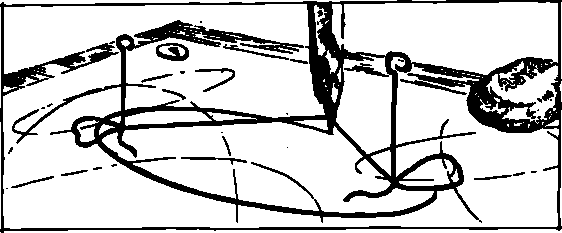
\includegraphics[width=\textwidth]{figures/fig-6-5.pdf}
 \caption{Drawing an ellipse.}
 \label{fig-6-5}
 \end{figure}


Ellipses can have various forms. If the thread is taken
much longer than the distance between the pins, then
the ellipse will be very similar to a circle. If, on the
contrary, the length of the thread barely exceeds the distance between the pins, then an elongated ellipse
-- almost a stick -- will be obtained.

A planet describes an ellipse at one of whose foci is
the Sun.

But what kind of ellipses do planets describe? It turns
out that they are very close to circles.

The path of the planet nearest to the Sun -- Mercury --
differs most from a circle. But even in this case, the
longest diameter of the ellipse is only 2\% greater than
the shortest one. The situation is different with the
orbits of artificial satellites. Take a look at \figr{fig-6-6}.

 \begin{figure}[!ht]
 \centering
 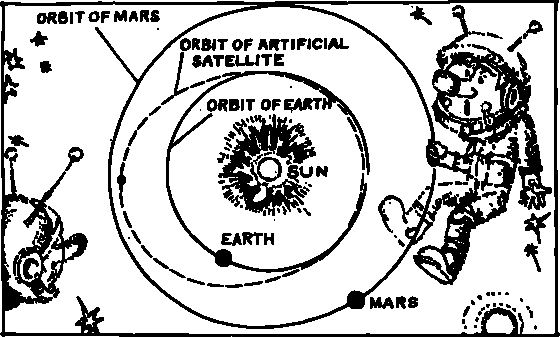
\includegraphics[width=\textwidth]{figures/fig-6-6.pdf}
 \caption{Orbits of planets are almost circles.}
 \label{fig-6-6}
 \end{figure}

You can't distinguish the orbit of Mars from a circle.
However, since the Sun is located at one of the foci
of the ellipse and not at its centre, the distance of a planet
from the Sun changes more noticeably. Let us draw a line
through the two foci of an ellipse. This line intersects
the ellipse at two places. The point nearest to the Sun
is called the perihelion, the farthest from the Sun the
aphelion. Mercury, when located at the perihelion, is
1.5 times closer to the Sun than at the aphelion.

The major planets describe ellipses around the Sun
which are close to circles. However, there are celestial
bodies which move around the Sun in greatly flattened
ellipses. Among them are comets. Their orbits are not
at all comparable with respect to elongation to those
of the planets. With regard to the celestial bodies moving
in ellipses it can be said that they belong to the solar
family. However, casual newcomers also drop in at our
system.

There have been observed comets describing curves
around the Sun whose forms suggest the following conclusion: the comet will not return; it does not belong to the
family of the solar system. The ``open'' curves described
by comets are called hyperbolas.

Such comets move especially fast when passing near
the Sun. This is understandable, since the total energy
of a comet is constant and, when approaching the Sun,
it has the minimum potential energy. Hence, its kinetic
energy is maximum at this time. Of course, such an
effect takes place for all the planets and for our Earth.
However, this effect is slight, since the difference in the
potential energies at the aphelion and perihelion is small.


 \begin{figure}[!ht]
 \centering
 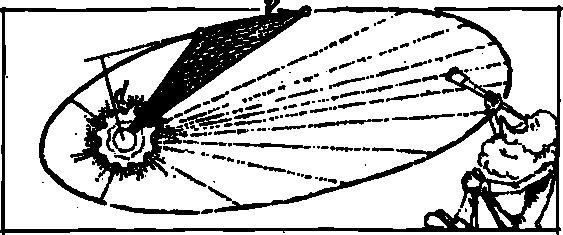
\includegraphics[width=\textwidth]{figures/fig-6-7.pdf}
 \caption{Planets sweep equal areas on equal amount of time.}
 \label{fig-6-7}
 \end{figure}


An interesting law of planetary motion follows from
the law of conservation of angular momentum.

Two positions of a planet are depicted in \figr{fig-6-7}.
From the Sun, i.e. from a focus of the ellipse, the two
radii are drawn to the two positions of the planet, and
the sector so formed is shaded. We are to determine the
area swept out by a radius in a unit of time. For a small
angle, the sector swept out by a radius in a second may
be replaced by a triangle. The base of the triangle is
the speed $v$ (the distance covered in a second), while
the altitude of the triangle is equal to the lever arm $d$
of the velocity. Therefore, the area of the triangle is $vd/2$.

The constancy of the quantity $mvd$ during the motion
follows from the law of conservation of angular momentum. But if $mvd$ is constant, so is the area of the triangle $vd/2$. We can draw sectors for any interval of time -- they
will turn out identical in area. The speed of a planet changes, but the so-called areal velocity remains constant.

Not all stars are surrounded by planetary systems. There are quite a few double stars in the sky. Two enormous celestial bodies revolve around each other.
 \begin{figure}[!ht]
 \centering
 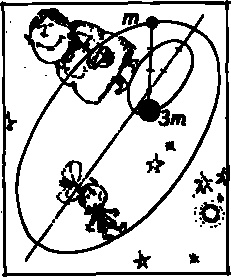
\includegraphics[width=0.45\textwidth]{figures/fig-6-8.pdf}
 \caption{Double stars revolve around their common centre of mass.}
 \label{fig-6-8}
 \end{figure}


The Sun's enormous mass makes it the centre of the
family. In double stars, both celestial bodies have masses
of the same order of magnitude. In this case, we may not
assume that one of the two stars is stationary. But how
does the motion proceed in this case? We know that each
closed system has one stationary (or uniformly moving)
point -- its centre of mass. Both the stars revolve around
this point. Moreover, they describe similar ellipses,
which follows from the condition written on p.~\pageref{ellipse},
$m_{1}/m_{2} = r_{2}/r_{1}$. The ellipse for one star is as many times greater than that for the other as the mass of one star
is less than that of the other \figr{fig-6-8}. In the case of
equal masses, both the stars will describe identical
trajectories around the centre of mass.

The planets of the solar system are in ideal conditions:
they are not subject to friction.

The small, artificial celestial bodies created by people -- satellites -- are not in such an ideal position: frictional
forces, however insignificant they may be at first, but none
the less perceptible, interfere decisively in their motion.

The total energy of a planet remains constant. The
total energy of a satellite falls slightly with every revolution. At first sight, it would seem that friction will slow down the motion of a -- satellite. In reality, the opposite occurs.

First of all, recall that the speed of a satellite is equal to $\sqrt{gR}$ or $\sqrt{GM/R}$, where $R$ is its distance from the
centre of the Earth, and $M$ its mass. The total energy of a satellite is equal to
 \begin{equation*}%
E =   - \, G \, \dfrac{M m}{R} +  \dfrac{mv^{2}}{2} 
 \end{equation*}
Substituting the value of the speed of the satellite,
we find the expression $GMm/2R$ for the kinetic energy.
We find that the magnitude of the kinetic energy is half
as great as that of the potential one, while the total
energy is equal to
 \begin{equation*}%
E = -\dfrac{G}{2} +  \dfrac{Mm}{R} 
 \end{equation*}
In the presence of friction, the total energy falls, i.e.
(since it is negative) its magnitude grows; the distance $R$
starts decreasing: the satellite descends. What happens
to the energy summands in this connection? The potential energy decreases (grows in its magnitude), the kinetic energy increases.

Nevertheless, the net change is negative, since the
potential energy decreases twice as fast as the kinetic
energy increases. Friction leads to a growth in the speed
of a satellite and not to a reduction.

It is now clear why a large launch vehicle outflies a small
satellite. The friction acting on a large rocket is greater.

\section{Interplanetary Travel}

We have already witnessed many trips to the Moon.
Automatic space probes and manned craft have landed
on its surface and then returned. Space probes travelled
to Mars and Venus. And soon the other planets will also
be visited and automatic stations and people will return
from their surface.

We now know the main laws governing interplanetary
travel, namely the principle of rocket motion and the
method of calculating the different speeds that a body
requires to orbit a celestial body and to escape its gravitational pull.

Let us take the trip to the Moon as an example. For
this we must aim the rocket at a point on the Moon's
orbit. The Moon must arrive at this point at the same
time as the rocket. The rocket may follow various trajectories, even a straight one. But it is essential that it
attain the Earth's escape velocity. We must also bear
in mind that different trajectories require different
amounts of fuel since fuel consumption depends on acceleration. Another factor is that flight time greatly depends
on initial velocity. If this is minimum, the trip will take
about five days, but if the velocity is increased by \SI{0.5}{\kilo\meter\per\second},
flight time decreases to 24 hours.

It may seem that to get to the Moon the rocket must
only reach the region of the Moon's attraction with zero
velocity. After that it will simply fall onto the Moon.
But such reasoning is erroneous, since when the rocket
has a zero velocity with respect to the Earth, its velocity
with respect to the Moon is the velocity of the Moon on its
orbit around the Earth but oppositely directed.

The illustration \figr{fig-6-9} shows the trajectory of a rocket launched at
point $A$ and the path of the Moon. We can imagine that
the region of the Moon's attraction moves along the same
path (in this region the only force that acts on the rocket
is the Moon's gravitational pull). When the rocket enters
this region at point $B$, the Moon is at point $C$ and has
a velocity $v_{M}$ equal to \SI{1.02}{\kilo\meter\per\second}. If at $B$ the velocity
of the rocket with respect to the Earth were zero, with
respect to the Moon it would be $-v_{M}$. The rocket most
certainly will miss the Moon.

\begin{figure}[!ht]
\centering
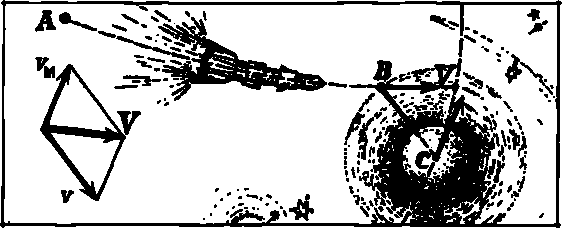
\includegraphics[width=\textwidth]{figures/fig-6-9.pdf}
\caption{Trajectory of a rocket launched to the Moon.}
\label{fig-6-9}
\end{figure}

If we are observing the rocket from the Moon, we can
be certain that it will meet the Moon at a right angle
if its velocity is $v$. What, then, should its optimal trajectory and velocity be? The rocket must obviously hit
point $B$ not with a zero velocity but with the velocity $V$
shown in the illustration \figr{fig-6-9}. For this we must simply use the
velocity parallelogram shown in the same figure.

We still have some leeway. Velocity vector $v$ does
not have to be pointed at the very centre of the Moon.
Besides, the gravitational pull of the Moon broadens
the error range.

Calculations show, however, that there is very little
elbowroom. The precision in initial velocity must be of
the order of several metres per second, and the angle at
which the rocket is launched must be set with an accuracy
of one-tenth of a degree and the timing of the launching
with an accuracy of several seconds.

So the rocket approaches the Moon with a non-zero velocity. Calculations show that this velocity, $V$, must be \SI{0.8}{\kilo\meter\per\second}. The Moon's gravitational pull makes the velocity greater and the rocket will collide with the Moon
at a velocity of \SI{2.5}{\kilo\meter\per\second}. This is no good of course, since the rocket would disintegrate at impact. The only solution is to lower the speed of descent by using braking rockets. The process of cushioning touchdown requires
a large supply of fuel. The formula on p.~\pageref{rocket-eq} shows that the rocket will ``lose weight'' by a factor of 2.7.

If we want the rocket to return to the Earth, it must have some fuel left. The Moon is a relatively small celestial body, only \SI{3476}{\kilo\meter} across and with a mass of \SI{7.34e22}{\kilo\gram}. We can easily see that its orbital velocity (i.e. the velocity required to maintain a satellite in an orbit around it) is \SI{1680}{\meter\per\second} and its escape velocity is \SI{2376}{\meter\per\second}, which means that to leave the Moon, the rocket must have a speed of about \SI{2.5}{\kilo\meter\per\second}. With this minimum initial speed the rocket will return to the Earth after five days and will have the familiar speed
of \SI{11}{\kilo\meter\per\second}.

The path of reentry into the Earth's atmosphere must
slope gently, since if there are astronauts inside the rocket
the forces of acceleration must be kept to a minimum.
But even if we are dealing with an automatic space probe,
the probe must make several revolutions around the
Earth so that the radius of its elliptical path decreases.
Then the reentry vehicle does not get overheated and can
safely return to the Earth.

Moon missions cost huge sums of money. If we assume
that the return pay-load of a manned flight to the Moon
is not less than 5 tons, then the total loaded weight at
lift-off must be about 4.5 thousand tons. Experts believe
that in the coming 20 years no more astronaut will visit
the Moon or, for that matter, any other planet. New
propulsion systems with greater exhaust velocities will
have to be constructed. However, one cannot be sure
of such predictions.

\section{If There Were No Moon}

We shall not discuss the sad consequences of the absence
of the Moon for poets and lovers. The title of this
section should be understood much more prosaically: how
the Moon's presence affects terrestrial mechanics.

In our previous discussion of what forces act on a book
lying on a table, we confidently stated: the Earth's
gravity and the reaction force. But, strictly speaking,
a book lying on a table is also attracted by the Moon,
the Sun and even the stars.

The Moon is our nearest neighbour. Let us forget about
the Sun and the stars and consider how much the weight
of a body on the Earth will change under the influence of
the Moon.

The Earth and the Moon are in relative motion, with
respect to the Moon the Earth as a whole (i.e. all points
of the Earth) is moving with an acceleration $Gm/r^{2}$,
where $m$ is the mass of the Moon, and $r$ is the distance
from the centre of the Moon to that of the Earth.

Consider a body lying on the Earth's surface. We are
interested in how much its weight will change owing
to the Moon's action. Terrestrial weight is determined
by acceleration with respect to the Earth. In other words,
we are therefore interested in how much the acceleration
with respect to the Earth of a body lying on the Earth's
surface will be changed by the Moon's action.

The acceleration of the Earth with respect to the Moon
is $Gm/r^{2}$; the acceleration with respect to the Moon of
a body lying on the Earth's surface is $Gm/r_{1}^{2}$, where $r_{1}
$ is the distance from the body to the centre of the Moon
\figr{fig-6-10}.

\begin{figure}[!ht]
\centering
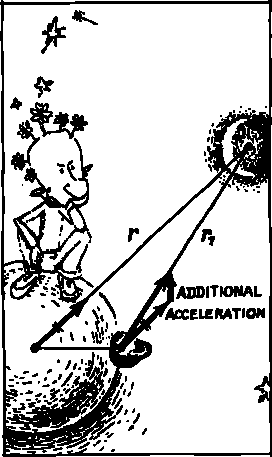
\includegraphics[width=0.45\textwidth]{figures/fig-6-10.pdf}
\caption{Acceleration of Earth with respect to the Moon.}
\label{fig-6-10}
\end{figure}

But we should find the additional acceleration of the
body with respect to the Earth: it will be equal to the
geometrical difference between the appropriate accelerations.

The value of  $Gm/r^{2}$ is a constant number for the Earth, while the value of  $Gm/r_{1}^{2}$ is different at various points on
the Earth's surface. Hence, the geometrical difference of interest to us will differ at various places on the Earth.
What will the terrestrial weight be at the place nearest
to the Moon, farthest from it and half-way along the
Earth's surface?



\begin{figure}[!ht]
\centering
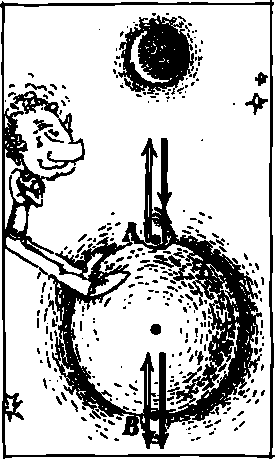
\includegraphics[width=0.45\textwidth]{figures/fig-6-11.pdf}
\caption{Finding acceleration induced due to the Moon.}
\label{fig-6-11}
\end{figure}

To find the acceleration with respect to the centre of
the Earth induced by the Moon on a body, i.e. the correction to the terrestrial gt it is necessary to subtract the
constant value of $Gm/r^{2}$ from the value of $Gm/r_{1}^{2}$ at the indicated places on the Earth (light arrows in \figr{fig-6-11}).

Moreover, it should be remembered that the acceleration
$Gm/r^{2}$ -- the acceleration of the Earth with respect to the
Moon -- is directed parallel to the line joining their
centres. The subtraction of a vector is equivalent to the
addition of the inverse vector. The vectors -- $Gm/r^{2}$ are
shown by means of bold-face arrows in the figure.

Adding the vectors depicted in the figure, we find what
we are interested in: the change in the acceleration of
free fall on the Earth's surface arising as a result of the
influence of the Moon.

At the place nearest to the Moon, the resulting additional acceleration will be equal to
 \begin{equation*}%
 G  \, \dfrac{m}{(r - R)^{2}} - G \, \dfrac{m}{r^{2}} 
 \end{equation*}
and directed towards the Moon. Earth's gravity diminishes; a body at point $A$ becomes lighter than in the
absence of the Moon.

Bearing in mind that $R$ is much smaller than $r$ , we are able to simplify the formula written above. Reducing
to a common denominator, we obtain:
 \begin{equation*}%
   \dfrac{GmR \, (2r - R)}{r^{2}(r - R)^{2}} 
 \end{equation*}
Discarding from the parentheses the relatively small
magnitude $R$ subtracted from the much larger magnitudes
$r$ or $2r$, we obtain
 \begin{equation*}%
   \dfrac{2GmR}{r^{3}} 
 \end{equation*}
 Let us now transfer to the antipode. At point $B$ the acceleration of a body due to the Moon isn't greater, but less than the total acceleration of the Earth. But we are now at the farthest side of the Earth from the Moon. A decrease in the Moon's attraction at this side of the Earth leads to the same result as an increase in the attraction at point $A$ -- to a decrease in the acceleration of free
fall. An unexpected result, isn't it? Here too a body becomes lighter under the action of the Moon. The difference
 \begin{equation*}%
G \,  \dfrac{m}{(r+ R)^{2}}  - G \, \dfrac{m}{r^{2}} \approx - \dfrac{2GmR}{r^{3}}
 \end{equation*}
turns out to be the same in absolute value as at point $A$.
\begin{figure}[!ht]
\centering
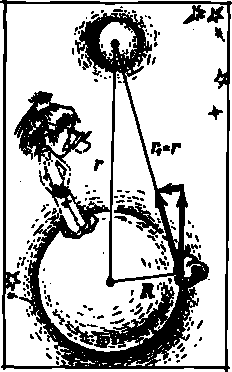
\includegraphics[width=0.45\textwidth]{figures/fig-6-12.pdf}
\caption{Finding acceleration induced due to the Moon.}
\label{fig-6-12}
\end{figure}

Things are different at the median line. Here the accelerations are directed at an angle to each other, and so
the subtraction of the total acceleration $Gm/r^{2}$ of the
Earth by the Moon and the acceleration $Gm/r_{1}^{2}$ of a body
lying on the Earth by the Moon must be carried out
geometrically \figr{fig-6-12}. We shall depart insignificantly from the median line if we place the body on the
Earth in such a way that $r_{1}$ and $r$ are equal in magnitude. The vector difference between the accelerations is the
base of an isosceles triangle. From the similarity of the triangles depicted in the diagram \figr{fig-6-12}, it is obvious that the
required acceleration is as many times less than $Gm/r^{2}$ as $R$ is less than $r$. Consequently, the required addition
to $g$ at the median line on the Earth's surface equals
\begin{equation*}%
\dfrac{GmR}{r^{3}}
 \end{equation*}
in magnitude this is one-half of the weakening of the
Earth's force of attraction at the extreme points. As for
the direction of this additional acceleration, it again
practically coincides, as can be seen from the figure,
with the vertical at the given point on the Earth's surface.
It is directed downwards, i.e. leads to an increase in
weight.

Thus, the influence of the Moon on terrestrial mechanics consists in a change in weight of bodies located on
the Earth's surface. Moreover, weight diminishes at the
nearest and farthest points from the Moon, but grows
on the median line, this change in weight in the latter
case being half as great as in the former.

Of course, the reasoning carried out is valid for any planet, for the Sun or for a star.

It is not difficult to calculate that neither planets nor
stars give even an insignificant fraction of the lunar
acceleration.

It is very easy to compare the action of any celestial body with that of the Moon: we must divide the additional acceleration due to this body by the lunar acceleration:

\begin{equation*}%
\dfrac{GmR}{r^{3}} : \dfrac{Gm_{M}R}{r_{M}^{3}}  = \dfrac{m}{m_{M}}  \dfrac{r^{3}_{M}}{r^{3}} 
 \end{equation*}
This product will fail to be much less than unity only
for the Sun. The Sun is much farther from us than the
Moon, but the mass of the Moon is tens of millions of
times less than that of the Sun.

Substituting numerical values, We find that under the
influence of the Moon terrestrial weight is changed 2.17
times as much as under that of the Sun.

Let us now estimate by how much the weight of terrestrial bodies would be changed if the Moon were to leave
its orbit around the Earth. Substituting numerical
values in the expression $2GmR/r^{3}$, we find that the lunar
acceleration is of the order of magnitude of \SI{0.0001}{\centi\meter\per\second\squared},
i.e. of one-ten-millionth of $g$.

Almost nothing, it would seem. Was it worthwhile
to follow with strained attention the solution to a rather
complicated mechanical problem for the sake of such
an insignificant effect? Don't hurry with such a conclusion. This ``insignificant'' effect is the cause of powerful tidal waves. It creates \SI{d15}{\joule} of kinetic energy daily, moving enormous masses of water. This energy equals that borne by all the Earth's rivers.

In fact, the percentage wise change in the quantity we computed is very small. A body which becomes lighter by such an ``insignificant'' amount will move a bit farther away from the centre of the Earth. But the radius of the Earth is \SI{6000000}{\meter}, and an insignificant deviation will be measured in tens of centimetres.

Imagine that the Moon stopped its motion relative
to the Earth and is shining somewhere over an ocean.
Calculations show that the water level at this place
would rise by  \SI{54}{\centi\meter}. Such a jump in the water level
would also occur at the antipode. On the median line
between these extreme points, the water level in the
ocean would drop by \SI{27}{\centi\meter}.

Thanks to the Earth's rotation about its axis, the
``places'' of rises and falls in the ocean are moving all the
time. These are tides. During about six hours, a rise
in the water level takes place and the water moves up
the shore -- this is high tide. Then low tide sets in; it
also lasts six hours. Two high tides and two low tides
occur every lunar day. The picture of tidal phenomena
is greatly complicated by the friction of water particles,
the form of the sea bottom and the contour of the shores.
For example, tides are impossible in the Caspian Sea
simply because the entire surface of the sea is subject
to the same conditions.

Tides are also absent from internal seas connected to
an ocean by long and narrow straits, for example, the
Black and Baltic seas.

Especially big tides occur in narrow bays, where a tidal
wave coming in from the ocean rises steeply. For example,
in the Gizhiginskaya Inlet on the Sea of Okhotsk, the
height of waves attains several metres.

If the ocean shore is sufficiently flat (for example, in
France), the rise of water during high tide can change the
location of the boundary between land and sea by many
kilometres.

Tidal phenomena hinder the Earth's rotation, for the
motion of tidal waves is related to friction. Work must
be expended to overcome this friction -- it is called tidal.
Therefore, the rotational energy, and with it the Earth's
rotational speed about its axis, falls.

This phenomenon leads to the lengthening of the day,
which was discussed on p. \pageref{longer-day}.

Tidal friction enables us to understand why one and
the same side of the Moon always faces the Earth.
At one time, the Moon was probably in a liquid state.
The rotation of this liquid sphere about the Earth was
accompanied by strong tidal friction, which gradually
slowed down the motion of the Moon. Finally, the Moon
stopped rotating with respect to the Earth, the tides
ceased and the Moon hid half of its surface from our
sight.
